% Biên dịch: xelatex report.tex (chạy 2 lần để cập nhật mục lục)
\documentclass[11pt,a4paper]{article}
\usepackage{fontspec}
\setmainfont{Times New Roman}
\setsansfont{Arial}
\setmonofont{Consolas}
\usepackage[a4paper,margin=2.3cm]{geometry}
\usepackage{amsmath,amssymb}
\usepackage{graphicx}
\usepackage{booktabs,tabularx,array}
\usepackage{xcolor}
\usepackage{enumitem}
\usepackage{caption}
\usepackage{float}
\usepackage[colorlinks=true,linkcolor=blue!50!black,citecolor=blue!50!black,urlcolor=blue!50!black]{hyperref}

\setlist{itemsep=2pt,topsep=4pt}
\renewcommand{\arraystretch}{1.25}
\newcolumntype{Y}{>{\raggedright\arraybackslash}X}
\captionsetup{font=small,labelfont=bf}

\definecolor{paper}{HTML}{2D5BE3}
\definecolor{nhom}{HTML}{B5521A}
\newcommand{\papersays}{\par\smallskip\noindent\textbf{\color{paper}Nội dung chính.}~}
\newcommand{\wesay}{\par\smallskip\noindent\textbf{\color{nhom}Nhận xét.}~}
\newcommand{\info}[1]{\par\noindent\textit{#1}\par\smallskip}
\newcommand{\metric}[1]{\texttt{#1}}

\title{\textbf{Định lượng và phân tích hiện tượng floater trong 3D Gaussian Splatting\\với số lượng góc nhìn hạn chế và sai lệch trắc quang giữa các ảnh}\\[4pt]
\large Báo cáo: Phát biểu bài toán và Tổng quan các công trình liên quan\\
\normalsize (Quantifying and Analyzing Floaters in Sparse-View 3DGS under Photometric Inconsistency)}
\author{Nhóm FaithfulRecon --- Trường Đại học Bách khoa, ĐHQG-HCM\\
GVHD: TS. Nguyễn Đức Dũng, ThS. Nguyễn Tuấn Khôi}
\date{Bản nháp sửa đổi lần 3, 14/11/2026}

\begin{document}
\maketitle

\begin{abstract}
\noindent Báo cáo trình bày cơ sở lý thuyết, phát biểu bài toán và tổng quan tài liệu cho đề tài nghiên cứu hiện tượng floater trong 3D Gaussian Splatting (3DGS) khi số lượng góc nhìn huấn luyện hạn chế và các ảnh huấn luyện chịu sai lệch trắc quang theo từng ảnh (phơi sáng, cân bằng trắng, ánh xạ tông màu). Câu hỏi nghiên cứu trung tâm là: \emph{độ phủ đa góc nhìn hạn chế và sai lệch trắc quang giữa các góc nhìn tác động riêng rẽ và đồng thời như thế nào đến sự hình thành các Gaussian nằm ngoài bề mặt.} Mục~\ref{sec:background} trình bày mô hình 3DGS và hai giả định nền tảng. Mục~\ref{sec:problem} xác định phạm vi thuật ngữ, phân tích hai nguồn gốc của floater, phân loại mức độ bằng chứng hiện có và nêu giả thuyết về cơ chế tương tác. Mục~\ref{sec:rw} phân tích 18 công trình liên quan. Mục~\ref{sec:gap} xác định các khoảng trống nghiên cứu và đóng góp dự kiến. Mục~\ref{sec:pilot} trình bày giao thức đo, kết quả sơ bộ và các yếu tố gây nhiễu đã nhận diện.

\smallskip\noindent\textbf{Quy ước trình bày.} Với mỗi công trình, phần \textcolor{paper}{\textbf{Nội dung chính}} tóm tắt những gì bài báo trình bày, kèm vị trí tham chiếu; phần \textcolor{nhom}{\textbf{Nhận xét}} là đánh giá của nhóm. Các nhận định được phân thành ba mức: \emph{có cơ sở} (được mô hình hoặc tài liệu hỗ trợ), \emph{giả thuyết} (hợp lý, có thể kiểm chứng, chưa được kiểm chứng) và \emph{chưa chặt chẽ}. Thông tin hội nghị được ghi theo bản PDF hoặc arXiv mà nhóm sử dụng.

\smallskip\noindent\textbf{Thay đổi so với bản trước.} (1) Thu hẹp phạm vi từ ``chiếu sáng không đồng nhất'' sang ``sai lệch trắc quang theo từng ảnh''; (2) phát biểu lại giả định A1, A2; (3) phát biểu thận trọng hơn giả thuyết cơ chế; (4) bổ sung Gaussian-DK, AD-GS, ICO-GS và bảng phân loại mức độ bằng chứng; (5) xác định lại khoảng trống và đóng góp; (6) định nghĩa đầy đủ chỉ số $W_{\text{float}}$ và các yếu tố gây nhiễu của thí nghiệm; (7) bổ sung kết quả E5 (SH bậc 3), E4 (bù affine theo ảnh), E1 (nhiễu theo pixel), E3 (lưới $N\times S$), kết quả kiểm tra scan24 và vấn đề của bề mặt tham chiếu (Mục~\ref{sec:factors}). Kết quả chính mới: P2 không được ủng hộ, vì trong khoảng $N=4$--8 tác động của sai lệch trắc quang tăng theo $N$; floater do thành phần sai lệch nhất quán trong từng ảnh gây ra, và bù affine theo ảnh không loại bỏ được floater.
\end{abstract}

\tableofcontents
\newpage

%=====================================================================
\section{Cơ sở lý thuyết}
\label{sec:background}

\subsection{Mô hình biểu diễn và quá trình kết xuất}
3D Gaussian Splatting biểu diễn cảnh bằng tập hợp $N$ hàm Gaussian ba chiều. Gaussian thứ $i$ được tham số hoá bởi tâm $\mu_i\in\mathbb{R}^3$, ma trận hiệp phương sai $\Sigma_i = R_iS_iS_i^\top R_i^\top$, độ mờ (opacity) $o_i$ và màu $c_i(\mathbf{d})$ phụ thuộc hướng nhìn $\mathbf{d}$, biểu diễn bằng các hệ số điều hoà cầu (spherical harmonics, SH). Màu tại pixel $\mathbf{p}$ được tính bằng phép trộn alpha các Gaussian theo thứ tự độ sâu:
\begin{equation}
\hat C(\mathbf{p}) = \sum_{i=1}^{K} c_i\,\alpha_i \prod_{j<i}(1-\alpha_j), \qquad
\alpha_i = o_i\,\exp\!\left(-\tfrac12(\mathbf{p}-\mu'_i)^\top \Sigma_i'^{-1}(\mathbf{p}-\mu'_i)\right),
\label{eq:blend}
\end{equation}
trong đó $\mu'_i$, $\Sigma'_i$ là tâm và hiệp phương sai sau phép chiếu. Đại lượng $w_i(\mathbf{p})=\alpha_i\prod_{j<i}(1-\alpha_j)$ là \emph{trọng số trộn}, biểu thị mức đóng góp của Gaussian $i$ vào pixel $\mathbf{p}$.

\subsection{Bài toán tối ưu}
Cho $n$ ảnh huấn luyện $\{I_k\}_{k=1}^n$ với tham số camera đã biết, tham số $\Theta$ được tối ưu theo hàm mất mát trắc quang
\begin{equation}
\mathcal{L}(\Theta) = \sum_{k=1}^{n} \mathcal{L}_k, \qquad
\mathcal{L}_k = (1-\lambda)\,\lVert \hat I_k(\Theta) - I_k\rVert_1 + \lambda\,\mathcal{L}_{\text{D-SSIM}}(\hat I_k(\Theta), I_k).
\label{eq:loss}
\end{equation}
Bên cạnh tối ưu theo gradient, 3DGS sử dụng cơ chế điều khiển mật độ thích nghi: tách hoặc nhân bản các Gaussian có gradient vị trí lớn (mật độ hoá), loại bỏ Gaussian có độ mờ thấp (cắt tỉa) và định kỳ khởi tạo lại độ mờ. Cơ chế này rời rạc, không khả vi; nghiệm cuối phụ thuộc đáng kể vào khởi tạo (MS-GS~\cite{msgs} §3.1) và vào tính ngẫu nhiên của mật độ hoá (AD-GS~\cite{adgs} §1).

\subsection{Hai giả định nền tảng}
\label{sec:assumptions}
\begin{enumerate}[label=\textbf{A\arabic*.}]
  \item \textbf{Độ phủ hình học đa góc nhìn đầy đủ} (sufficient multi-view geometric coverage). Mỗi vùng bề mặt được quan sát từ đủ số góc nhìn, với baseline và phân bố không gian phù hợp. Số lượng ảnh \emph{không đồng nhất} với độ phủ: nhiều ảnh chụp gần cùng vị trí có thể cung cấp ít ràng buộc hình học hơn số ít ảnh có baseline tốt. Trong thực nghiệm, số góc nhìn $N$ là biến độc lập chính, với điều kiện cách lấy mẫu camera được cố định (Mục~\ref{sec:protocol}).
  \item \textbf{Nhất quán trắc quang dưới điều kiện ngoại hình và chiếu sáng cố định}, sai khác giữa các góc nhìn chỉ đến từ các hiệu ứng phụ thuộc hướng nhìn đã được mô hình hoá (thành phần SH). Phát biểu này phân biệt sai khác \emph{được mô hình hoá} (phản xạ phụ thuộc hướng nhìn) với sai khác \emph{không được mô hình hoá} (ISP khác nhau giữa các ảnh, thay đổi chiếu sáng vật lý, bóng đổ thay đổi).
\end{enumerate}
Khi A1 và A2 được thoả mãn, ràng buộc đa góc nhìn trong~\eqref{eq:loss} loại trừ phần lớn các cấu hình hình học sai. Đây là một mô hình đơn giản hoá: ngay cả khi A1, A2 thoả mãn, 3DGS vẫn có thể sinh floater do khởi tạo và mật độ hoá~\cite{adgs}.

%=====================================================================
\section{Phát biểu bài toán}
\label{sec:problem}

\subsection{Phạm vi thuật ngữ}
\label{sec:terms}
Các khái niệm sau có liên quan nhưng không đồng nhất; báo cáo sử dụng chúng theo nghĩa trong Bảng~\ref{tab:terms}.

\begin{table}[H]
\centering\small
\caption{Phân biệt các loại sai lệch giữa các ảnh.}
\label{tab:terms}
\begin{tabularx}{\textwidth}{@{}l Y l@{}}
\toprule
Hiện tượng & Bản chất & Phạm vi đề tài \\
\midrule
Sai lệch phơi sáng (exposure) & Hệ số khuếch đại toàn ảnh khác nhau & Có \\
Sai lệch cân bằng trắng (white balance) & Hệ số theo kênh màu khác nhau & Có \\
Sai lệch ánh xạ tông màu / gamma & Đường cong cường độ khác nhau & Có (dạng toàn cục) \\
Thay đổi chiếu sáng vật lý (illumination) & Nguồn sáng thay đổi; bóng đổ và vùng phản xạ thay đổi theo không gian & Không (giai đoạn sau) \\
Sai lệch ngoại hình (appearance) & Khái niệm tổng quát, bao gồm tất cả các loại trên và thay đổi cảnh & Không \\
\bottomrule
\end{tabularx}
\end{table}

Thí nghiệm hiện tại mô phỏng ba dòng đầu bằng phép biến đổi toàn ảnh $I'_k=\operatorname{clip}(g_k\,\mathbf{w}_k\odot I_k)^{\gamma_k}$. Phép biến đổi này không tái hiện bóng đổ hay phản xạ thay đổi theo vị trí nguồn sáng. Do đó, đề tài sử dụng thuật ngữ \textbf{sai lệch trắc quang theo từng ảnh} (per-view photometric inconsistency caused by exposure, white balance and tone mapping), không khẳng định bao quát mọi trường hợp chiếu sáng không đồng nhất.

\subsection{Định nghĩa floater}
\emph{Floater} là các Gaussian nằm trong không gian trống, không thuộc bề mặt thực của vật thể; trên ảnh tổng hợp tại góc nhìn mới, chúng xuất hiện dưới dạng vệt mờ, mảng màu hoặc lớp nhiễu. Các công trình sử dụng nhiều thuật ngữ cho các hiện tượng liên quan: ``floater'' và ``background collapse''~\cite{fnm,sparsegs}, ``bright/dark blobs''~\cite{vastgaussian}, ``black or white splats''~\cite{gaussiandk}, ``elongated artifacts''~\cite{sparsegsw}.

Phần lớn công trình chỉ minh hoạ floater định tính và đánh giá bằng chỉ số ảnh. Floater là sai số hình học; chỉ số ảnh chỉ phản ánh nó gián tiếp. Đề tài đo floater thông qua khoảng cách tới bề mặt tham chiếu của DTU. Cần lưu ý rằng khoảng cách từ \emph{tâm} Gaussian tới bề mặt là một \emph{đại lượng thay thế} (proxy) cho floater, không phải định nghĩa tuyệt đối: Gaussian có tâm lệch nhưng hiệp phương sai lớn vẫn có thể bao phủ bề mặt, và ngược lại (Mục~\ref{sec:metric-limits}).

\subsection{Nguồn gốc thứ nhất: độ phủ đa góc nhìn hạn chế}
\begin{itemize}
  \item \textbf{Tính đa nghiệm của phép chiếu:} nghiệm tối ưu quá khớp với các góc nhìn huấn luyện (SparseGS~\cite{sparsegs} §1; FSGS~\cite{fsgs} §1).
  \item \textbf{Mật độ hoá không kiểm soát:} Gaussian mới sinh từ phép tách được lấy mẫu không ràng buộc, có thể nằm sai vị trí; khi ít ảnh, cắt tỉa không loại bỏ được chúng, và \emph{màu của floater được điều chỉnh để khớp các ảnh huấn luyện} thay vì floater bị loại bỏ (AD-GS~\cite{adgs} §1, §3).
  \item \textbf{Ngoại hình bù trừ cho hình học thiếu ràng buộc:} với ít quan sát, giám sát trắc quang độc lập theo từng ảnh cho phép thành phần ngoại hình quá khớp từng góc nhìn bằng cách bù trừ sai số hình học (ICO-GS~\cite{icogs} §1).
  \item \textbf{Mất cân bằng gradient gần camera} (NeRF): Floaters No More~\cite{fnm} §1, §4.
\end{itemize}

\subsection{Nguồn gốc thứ hai: sai lệch trắc quang giữa các ảnh}
Khi các phép biến đổi $\phi_k$ của từng ảnh khác nhau, không tồn tại trường màu 3D nhất quán tái tạo chính xác toàn bộ $\{I'_k\}$; giả định A2 bị vi phạm. Các công trình ghi nhận:
\begin{itemize}
  \item Gaussian-DK~\cite{gaussiandk} (§3.3, §5.2.3): floater của 3DGS là các Gaussian bù trừ sai khác độ sáng giữa các góc nhìn nhưng không phù hợp với hình học cảnh; các Gaussian này nằm xa tâm cảnh để giảm ảnh hưởng tới góc nhìn khác, do đó thường ở gần camera.
  \item VastGaussian~\cite{vastgaussian} (§1, Hình~2): vùng Gaussian sáng/tối hình thành gần camera của ảnh phơi sáng mạnh/yếu.
  \item Bilateral Guided RF~\cite{bilarf} (§1, Hình~2): xử lý ISP khác nhau gây floater, kể cả với ảnh chụp ở chế độ tự động.
  \item ICO-GS~\cite{icogs} (§1): thay đổi chiếu sáng, che khuất và vùng chỉ một góc nhìn quan sát vi phạm giả định nhất quán trắc quang.
\end{itemize}

\subsection{Phân loại mức độ bằng chứng hiện có}
\label{sec:evidence}
\begin{table}[H]
\centering\small
\caption{Trạng thái bằng chứng của các mệnh đề liên quan.}
\label{tab:evidence}
\begin{tabularx}{\textwidth}{@{}Y Y@{}}
\toprule
Mệnh đề & Trạng thái bằng chứng \\
\midrule
Sai lệch trắc quang làm suy giảm chất lượng tái tạo của NeRF/3DGS & Có cơ sở: nhiều công trình~\cite{nerfw,vastgaussian,bilarf,gaussiandk,luminancegs} \\
Ít góc nhìn làm hình học thiếu ràng buộc và dễ xuất hiện floater & Có cơ sở~\cite{sparsegs,fsgs,corgs,adgs,icogs} \\
Floater được hình thành hoặc duy trì để khớp ảnh huấn luyện & Đã được phân tích~\cite{adgs,icogs} \\
Sai lệch trắc quang trực tiếp làm tăng floater & Có bằng chứng gợi ý: Gaussian-DK nêu dưới dạng giả định, kèm hình định tính, trên dữ liệu dày; chưa có thí nghiệm cô lập nguyên nhân \\
Ít góc nhìn và sai lệch trắc quang \emph{tương tác} làm tăng floater vượt tác động riêng lẻ & Chưa có bằng chứng thực nghiệm dạng giai thừa trong các công trình đã khảo sát \\
\bottomrule
\end{tabularx}
\end{table}
Hệ quả: đề tài \textbf{không} đặt đóng góp là phát hiện rằng sai lệch trắc quang gây floater. Đóng góp được đặt vào việc \emph{định lượng} tác động riêng rẽ và tương tác của hai yếu tố bằng chỉ số hình học.

\subsection{Giả thuyết về cơ chế}
\label{sec:mechanism}
Mục này trình bày giả thuyết, chưa phải kết luận.

\paragraph{Hai cơ chế giảm phần dư trắc quang.} Ký hiệu $r_k = I'_k - \hat I_k$. Khi các $\phi_k$ khác nhau, $r_k$ chứa thành phần hệ thống $\Delta_k$ không giải thích được bằng một trường màu nhất quán. Mô hình có thể giảm $\Delta_k$ bằng (a) điều chỉnh màu phụ thuộc hướng nhìn của Gaussian trên bề mặt (thành phần SH bậc $\ge 1$); hoặc (b) hình thành các Gaussian ngoài bề mặt: do thị sai, mỗi Gaussian như vậy đóng góp lên các pixel khác nhau và che các điểm bề mặt khác nhau ở từng góc nhìn, tạo ra sai khác ngoại hình phụ thuộc góc nhìn bằng hình học. Gaussian-DK~\cite{gaussiandk} (§3.3) nêu một giả định tương tự cho cơ chế (b) trên dữ liệu dày.

\paragraph{Lưu ý về biểu diễn màu trong thí nghiệm.} Mã nguồn của nhóm sử dụng màu RGB không phụ thuộc hướng nhìn (SH bậc 0), khác với 3DGS chuẩn (SH bậc 3). Với SH bậc 0, cơ chế (a) không tồn tại; sai khác phụ thuộc góc nhìn chỉ có thể được tạo bằng hình học. Do đó kết quả hiện tại có thể \emph{đánh giá cao hơn} tác động của sai lệch trắc quang so với 3DGS chuẩn. Thí nghiệm E5 (SH bậc 3) được thiết kế để kiểm tra điểm này. Kết quả E5 (Mục~\ref{sec:robust}) cho thấy floater vẫn tăng theo $S$ khi có SH bậc 3 (giữ 54--95\% mức tăng); do đó việc thiếu kênh màu phụ thuộc hướng nhìn không đủ để giải thích hiện tượng.

\paragraph{Vai trò của độ phủ đa góc nhìn.} Phát biểu thận trọng: \emph{khi độ phủ đa góc nhìn giảm, thể tích các vùng không gian có ràng buộc quan sát yếu tăng lên; trong các vùng này, mô hình có khả năng cao hơn hình thành Gaussian ngoài bề mặt để giải thích phần dư trắc quang riêng của từng góc nhìn.} Phát biểu này có các điều kiện sau:
\begin{itemize}
  \item Quan hệ ``ít góc nhìn hơn thì vùng ràng buộc yếu lớn hơn'' chỉ được bảo đảm khi các tập camera \emph{lồng nhau}. Thiết kế thí nghiệm của nhóm thoả điều kiện này (Mục~\ref{sec:protocol}); không thể khẳng định cho mọi cặp tập camera bất kỳ.
  \item Gaussian có kích thước không gian và vùng chiếu (footprint) trên ảnh; khả năng quan sát còn phụ thuộc che khuất. Do đó, Gaussian có tâm nằm trong vùng chỉ một camera quan sát vẫn có thể nhận gradient từ camera khác.
  \item Cơ chế này không được giả định là nguyên nhân duy nhất của tương tác; mật độ hoá (AD-GS) và khởi tạo cũng ảnh hưởng.
\end{itemize}

\paragraph{Các dự đoán có thể kiểm chứng.}
\begin{itemize}
  \item[\textbf{P1.}] Với $N$ cố định, chỉ số floater tăng theo cường độ sai lệch trắc quang $S$.
  \item[\textbf{P2.}] Mức tăng trong P1 lớn hơn khi $N$ nhỏ hơn (tương tác).
  \item[\textbf{P3.}] Floater do sai lệch trắc quang tập trung phía trước bề mặt theo hướng nhìn camera.
  \item[\textbf{P4.}] Mức cải thiện chỉ số ảnh do mô-đun bù ngoại hình không nhất thiết đi kèm mức cải thiện hình học tương ứng. Đây là giả thuyết; không giả định rằng mô-đun nhiều tham số luôn hấp thụ sai số hình học.
\end{itemize}

\subsection{Câu hỏi nghiên cứu}
\begin{quote}
\emph{Độ phủ đa góc nhìn hạn chế và sai lệch trắc quang giữa các góc nhìn tác động riêng rẽ và đồng thời như thế nào đến sự hình thành các Gaussian nằm ngoài bề mặt trong 3DGS?}
\end{quote}
\begin{itemize}
  \item[\textbf{RQ1}] (đóng góp chính). Khi chỉ giảm $N$, khi chỉ tăng $S$, và khi đồng thời thay đổi cả hai, chỉ số floater hình học thay đổi như thế nào? Có tương tác giữa hai yếu tố không? (P1--P3)
  \item[\textbf{RQ2}] (thu hẹp). Với 1--2 mô-đun bù ngoại hình, quan hệ giữa mức cải thiện trắc quang, mức cải thiện hình học và dung lượng mô-đun là gì? Kèm một thí nghiệm kiểm tra độ tin cậy của rendering disagreement (CoR-GS) dưới sai lệch trắc quang hệ thống. (P4)
  \item[\textbf{RQ3}] (giai đoạn sau). Phát hiện và giảm floater do sai lệch trắc quang bằng tín hiệu chi phí thấp.
\end{itemize}

%=====================================================================
\section{Tổng quan các công trình liên quan}
\label{sec:rw}

Nhóm đã khảo sát 19 công trình, trong đó 18 công trình thuộc phạm vi đề tài (GSWAM, về thao tác robot, bị loại). Các công trình được phân thành ba nhóm (Bảng~\ref{tab:map}).

\begin{table}[H]
\centering\small
\caption{Phân loại các công trình liên quan.}
\label{tab:map}
\begin{tabularx}{\textwidth}{@{}l Y Y@{}}
\toprule
Nhóm & Công trình & Hướng tiếp cận chính \\
\midrule
A. Sparse-view (vi phạm A1) & Floaters No More~\cite{fnm}, SparseGS~\cite{sparsegs}, FSGS~\cite{fsgs}, DNGaussian~\cite{dngaussian}, CoR-GS~\cite{corgs}, AD-GS~\cite{adgs}, ICO-GS~\cite{icogs}, HeroGS~\cite{herogs} & Ràng buộc hình học: tiên nghiệm độ sâu, góc nhìn giả lập, cắt tỉa, đồng chính quy hoá, kiểm soát mật độ hoá \\
B. Ngoại hình (vi phạm A2) & NeRF-W~\cite{nerfw}, VastGaussian~\cite{vastgaussian}, Bilateral Guided RF~\cite{bilarf}, WildGaussians~\cite{wildgaussians}, Appearance Codes + Bilateral Grids~\cite{unifying}, Luminance-GS~\cite{luminancegs} & Tham số ngoại hình riêng cho từng ảnh \\
C. Liên quan trực tiếp tới floater và sai lệch trắc quang & Gaussian-DK~\cite{gaussiandk}, SparseGS-W~\cite{sparsegsw}, MS-GS~\cite{msgs}, WildSplatter~\cite{wildsplatter} & Xét đồng thời sai lệch giữa các ảnh và floater hoặc ít ảnh \\
\bottomrule
\end{tabularx}
\end{table}

%---------------------------------------------------------------------
\subsection{Nhóm A: tái tạo từ số lượng ảnh hạn chế}

\subsubsection{Floaters No More~\cite{fnm}}
\info{Philip, Deschaintre (Adobe Research), 2023. NeRF và các biến thể.}
\papersays
Background collapse do vùng gần camera có mật độ điểm lấy mẫu cao hơn nên nhận gradient lớn hơn (§1). Phương pháp nhân gradient điểm mẫu với $s_{\nabla p}=\min(1,(\delta_{ip})^2)$, $\delta_{ip}$ là khoảng cách tới gốc tia (Phương trình~4).
\wesay
Công trình đề xuất một cơ chế giải thích vị trí floater gần camera. Gaussian-DK~\cite{gaussiandk} kế thừa ý tưởng này cho 3DGS. Không xét yếu tố trắc quang.

\subsubsection{SparseGS~\cite{sparsegs}}
\info{Xiong và cộng sự, arXiv 2312.00206. Mip-NeRF 360 (12 ảnh), LLFF và DTU (3 ảnh).}
\papersays
Độ sâu softmax-scaling (Phương trình~5), ràng buộc Pearson với độ sâu đơn ảnh, Unseen Viewpoint Regularization dùng SDS, và cắt tỉa floater theo sai khác giữa độ sâu mode và độ sâu trộn alpha (§3.4).
\wesay
Tiêu chí cắt tỉa dựa trên độ sâu kết xuất; Gaussian bù trừ màu nằm sát trước bề mặt với trọng số lớn có thể không bị phát hiện. Đánh giá bằng PSNR, SSIM, LPIPS.

\subsubsection{FSGS~\cite{fsgs} và DNGaussian~\cite{dngaussian}}
\info{FSGS: ECCV 2024, LLFF, Mip-NeRF 360, Blender. DNGaussian: CVPR 2024, LLFF, DTU (3 góc nhìn), Blender.}
\papersays
FSGS bổ sung Gaussian bằng proximity-guided unpooling và ràng buộc độ sâu Pearson trên góc nhìn giả lập. DNGaussian dùng Hard/Soft Depth Regularization và Global-Local Depth Normalization; tác giả nêu trong phần hạn chế rằng ngoại hình không nhất quán tại vùng phản xạ vẫn là thách thức.
\wesay
Cả hai giả định A2; DNGaussian tự nhận diện A2 là điểm yếu nhưng không thực nghiệm trên dữ liệu sai lệch trắc quang.

\subsubsection{CoR-GS~\cite{corgs}}
\info{Zhang và cộng sự, ECCV 2024. LLFF, Mip-NeRF 360, DTU, Blender.}

\begin{figure}[H]
\centering
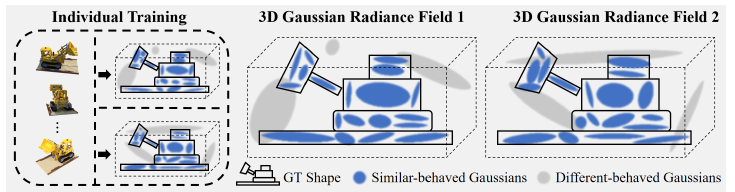
\includegraphics[width=0.72\textwidth]{figures/c_corgs.png}
\caption{Trích từ CoR-GS~\cite{corgs}, Fig.~1: Gaussian có hành vi khác nhau giữa hai trường huấn luyện độc lập thường không khớp hình dạng thực.}
\end{figure}

\papersays
Point disagreement (Fitness, RMSE với $\tau=5$) và rendering disagreement tương quan nghịch với độ chính xác tái tạo (§3); co-pruning loại Gaussian không có điểm tương ứng; đồng chính quy hoá trên góc nhìn nội suy.
\wesay
Giả định ngầm: sai số của hai trường ngẫu nhiên, độc lập. Với sai lệch trắc quang hệ thống, hai trường có thể cùng hình thành floater tại cùng vị trí, khi đó độ bất đồng không phản ánh sai số. Đây là giả thuyết được kiểm tra bằng một thí nghiệm riêng trong RQ2 (E7, Mục~\ref{sec:contrib}).

\subsubsection{AD-GS~\cite{adgs}}
\info{Patle, Girgaonkar, Somraj, Soundararajan (IISc, BITS Pilani). ACM TOG / SIGGRAPH Asia 2025, arXiv 2509.11003. Dữ liệu: LLFF, Tanks and Temples (3, 6, 9 góc nhìn) và các tập khác.}
\papersays
\begin{itemize}
  \item Nguyên nhân chính của floater khi ít ảnh là \emph{mật độ hoá không kiểm soát}: Gaussian mới từ phép tách được lấy mẫu không ràng buộc và có thể nằm sai vị trí, dẫn tới mật độ hoá tiếp quanh chúng (§1).
  \item Floater đã hình thành không bị hàm mất mát trắc quang loại bỏ; \emph{màu của floater được điều chỉnh để khớp các ảnh huấn luyện}, gây biến dạng ở góc nhìn mới (§3, Hình~2).
  \item Phương pháp luân phiên pha mật độ hoá mạnh (ngưỡng gradient thấp, chỉ mất mát trắc quang) và pha mật độ hoá yếu (cắt tỉa theo độ mờ với ngưỡng cao, ràng buộc pseudo-view giữa hai mô hình và độ trơn độ sâu theo biên).
\end{itemize}
\wesay
\begin{itemize}
  \item Kết luận ``mất mát trắc quang đổi màu floater thay vì loại bỏ'' hỗ trợ cơ chế (b) ở Mục~\ref{sec:mechanism} và giải thích vì sao floater tồn tại dai dẳng.
  \item Số Gaussian tăng khi sai lệch trắc quang tăng (Mục~\ref{sec:pilot}) có thể một phần do mật độ hoá phản ứng với gradient lớn hơn; cần phân tích thành phần này riêng.
  \item Thí nghiệm theo 3/6/9 góc nhìn nhưng không có sai lệch trắc quang; đánh giá bằng chỉ số ảnh.
\end{itemize}

\subsubsection{ICO-GS~\cite{icogs}}
\info{Xiong và cộng sự (Peking University, Peng Cheng Laboratory, Alibaba), CVPR 2026, arXiv 2603.02893. Dữ liệu: LLFF, DTU (3 góc nhìn), Blender.}
\papersays
\begin{itemize}
  \item Mỗi Gaussian có thuộc tính hình học và ngoại hình gắn liền. Với ít quan sát, giám sát trắc quang độc lập theo từng ảnh cho phép \emph{ngoại hình quá khớp từng góc nhìn bằng cách bù trừ sai số hình học}, trong khi hình học thiếu ràng buộc; kết quả là ảnh huấn luyện hợp lý nhưng góc nhìn mới có floater hoặc mờ (§1).
  \item Giả định nhất quán trắc quang bị vi phạm bởi thay đổi chiếu sáng, che khuất và vùng chỉ một góc nhìn quan sát; tác giả dùng ràng buộc nhất quán dựa trên đặc trưng để giảm ảnh hưởng của sai lệch chiếu sáng và ảnh (§1).
  \item Phương pháp: ràng buộc trắc quang đa góc nhìn với chọn top-$k$ theo pixel, độ trơn theo biên; lọc độ sâu nhất quán chu trình để tổng hợp góc nhìn ảo. Cải thiện khoảng 1.1 dB PSNR trên DTU 3 góc nhìn (đóng góp).
\end{itemize}
\wesay
Công trình cung cấp cơ sở lý thuyết cho nhận định ``ngoại hình bù trừ cho hình học thiếu ràng buộc'' (liên quan P4). ICO-GS không mô hình hoá sai lệch ngoại hình giữa các ảnh và không thực nghiệm với sai lệch trắc quang có kiểm soát.

\subsubsection{HeroGS~\cite{herogs}}
\info{Li và cộng sự (UCAS), arXiv 2603.01099 (2026).}
\papersays
Hướng dẫn ba cấp: nhãn giả bằng nội suy khung hình (cấp ảnh), FADP (cấp đặc trưng), co-pruning CPG (cấp tham số).
\wesay
Nhãn giả từ nội suy khung hình giả định ngoại hình liên tục giữa hai ảnh kề nhau; với sai lệch trắc quang, nhãn giả có ngoại hình trung gian.

\paragraph{Tổng kết nhóm A.} Các công trình sử dụng dữ liệu có điều kiện chụp được kiểm soát và đánh giá bằng chỉ số ảnh. AD-GS và ICO-GS phân tích cơ chế floater khi ít ảnh, trong đó thành phần ngoại hình bù trừ cho sai số hình học; không công trình nào đưa sai lệch trắc quang vào làm biến thực nghiệm.

%---------------------------------------------------------------------
\subsection{Nhóm B: mô hình hoá ngoại hình}

\subsubsection{NeRF-W~\cite{nerfw}}
\info{Martin-Brualla và cộng sự (Google), CVPR 2021. PhotoTourism, số lượng ảnh lớn.}
\papersays
Appearance embedding theo ảnh và trường transient. Embedding của ảnh kiểm tra được tối ưu trên nửa trái ảnh. Hạn chế: chất lượng suy giảm tại vùng ít được quan sát.
\wesay
Với giao thức nửa trái/nửa phải, PSNR phản ánh đồng thời hình học và khả năng tái tạo ngoại hình ảnh kiểm tra.

\subsubsection{VastGaussian~\cite{vastgaussian}}
\info{Lin và cộng sự, CVPR 2024. Cảnh quy mô lớn, số lượng ảnh lớn.}

\begin{figure}[H]
\centering
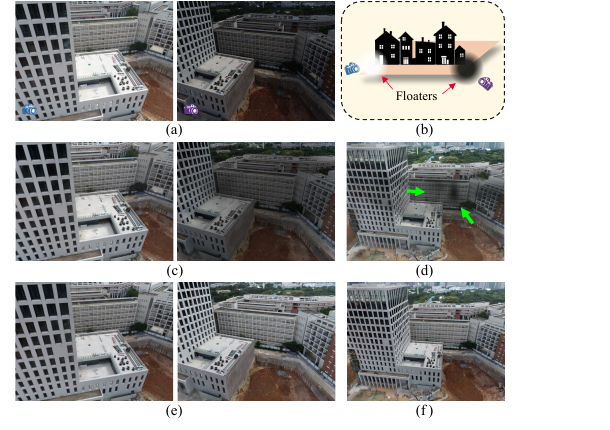
\includegraphics[width=0.56\textwidth]{figures/c_vast.png}
\caption{Trích từ VastGaussian~\cite{vastgaussian}, Fig.~2: vùng sáng/tối hình thành gần camera để khớp ảnh có độ phơi sáng khác nhau và trở thành floater tại góc nhìn mới; mô hình hoá ngoại hình tách rời làm giảm floater.}
\label{fig:vast}
\end{figure}

\papersays
Decoupled appearance modeling: CNN sinh transformation map từ ảnh kết xuất và embedding; mất mát trắc quang tính trên ảnh đã điều chỉnh, D-SSIM tính trên ảnh gốc; mô-đun bị loại bỏ sau huấn luyện (§4.3).
\wesay
Bằng chứng định tính cho cơ chế (b). Không đo floater; dữ liệu dày. Có thể dùng làm mô-đun bù ngoại hình dung lượng trung bình trong RQ2.

\subsubsection{Bilateral Guided RF~\cite{bilarf}}
\info{Wang và cộng sự (CUHK), SIGGRAPH 2024. Nền ZipNeRF, ảnh điện thoại, số lượng ảnh lớn.}
\papersays
Bilateral grid 3D theo góc nhìn (ma trận affine $3\times4$ mỗi ô) xấp xỉ ISP; ràng buộc TV; lưới $1\times1\times1$ suy biến thành affine toàn cục (§5). Sai lệch ISP nhỏ đủ gây floater (Hình~2).
\wesay
Độ phân giải lưới là trục dung lượng liên tục cho RQ2.

\subsubsection{WildGaussians~\cite{wildgaussians}}
\info{Kulhanek và cộng sự, NeurIPS 2024. PhotoTourism, NeRF On-the-go.}
\papersays
Embedding ảnh và Gaussian sinh biến đổi affine màu; 3DGS có thể loại bỏ vĩnh viễn hình học khi tín hiệu huấn luyện sai (§1, §3).
\wesay
MS-GS~\cite{msgs} §4.4 nhận định nhánh affine của WildGaussians hấp thụ sai số trắc quang khi ít ảnh.

\subsubsection{Appearance Codes + Bilateral Grids~\cite{unifying}}
\info{Wang và cộng sự, arXiv 2506.05280. Dữ liệu lái xe có LiDAR.}
\papersays
Multi-scale bilateral grid; hàm mục tiêu kết hợp mất mát ảnh và mất mát độ sâu LiDAR; đánh giá Chamfer Distance; cải thiện hình học do giảm floater gây bởi sai lệch trắc quang.
\wesay
Công trình duy nhất định lượng quan hệ bù ngoại hình -- hình học, nhưng có giám sát độ sâu trực tiếp và số lượng ảnh lớn.

\subsubsection{Luminance-GS~\cite{luminancegs}}
\info{Cui, Chu, Harada, CVPR 2025. Thiếu sáng, quá sáng, phơi sáng thay đổi.}
\papersays
Ma trận màu và đường cong tông màu theo góc nhìn; ràng buộc hình dạng đường cong.
\wesay
Mô hình biến đổi gần với mô hình nhiễu của nhóm; phù hợp làm mô-đun bù ngoại hình đối chứng.

\paragraph{Tổng kết nhóm B.} Các công trình bổ sung tham số ngoại hình theo ảnh với dung lượng khác nhau, đều sử dụng số lượng ảnh lớn và đánh giá chủ yếu bằng chỉ số ảnh.

%---------------------------------------------------------------------
\subsection{Nhóm C: liên quan trực tiếp tới floater và sai lệch trắc quang}

\subsubsection{Gaussian in the Dark (Gaussian-DK)~\cite{gaussiandk}}
\info{Ye, Dong, Hu, Wen, Liu (Tsinghua, Beijing Jiaotong). Pacific Graphics 2024, Computer Graphics Forum 43(7), arXiv 2408.09130. Dữ liệu: 12 cảnh tối tự thu (5 trong nhà, 7 ngoài trời), mỗi cảnh khoảng 80--130 ảnh sRGB chụp bằng iPhone 14 Pro ở chế độ phơi sáng tự động; khởi tạo bằng COLMAP.}

\begin{figure}[H]
\centering
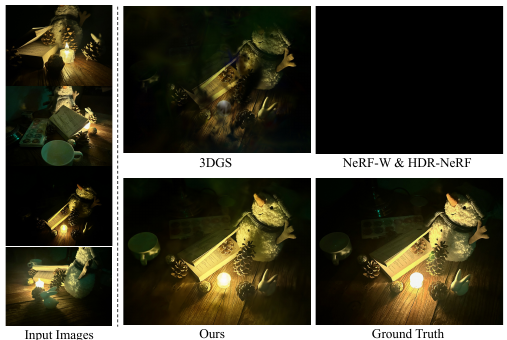
\includegraphics[width=0.6\textwidth]{figures/c_gdk.png}
\caption{Trích từ Gaussian-DK~\cite{gaussiandk}, Fig.~4: cảnh ``Snowman'' với góc nhìn và khoảng cách chụp thay đổi lớn. 3DGS sinh nhiều floater; NeRF-W và HDR-NeRF thất bại.}
\label{fig:gdk}
\end{figure}

\papersays
\begin{itemize}
  \item Ảnh chụp trong môi trường tối có sai khác độ sáng đáng kể giữa các góc nhìn; tác giả xác định nguyên nhân chủ yếu là \emph{quá trình tạo ảnh của camera} (phơi sáng tự động thay đổi theo vùng lấy nét), trong khi nguồn sáng của cảnh cố định (§1, §3).
  \item Camera response module: mức phơi sáng $\Delta E = K\,T\,\text{ISO}/A^2$ tính từ EXIF (Phương trình~5); đặc trưng ánh sáng gắn với từng Gaussian, kết xuất thành bản đồ đặc trưng và qua CNN để tạo bản đồ độ sáng theo pixel (Phương trình~6); tone-mapper CNN theo từng kênh màu trong miền logarit (Phương trình~7--9).
  \item \textbf{Floater} (§3.3): sau khi bổ sung camera response module, vẫn còn floater gần camera. Tác giả \emph{giả định} đây là các Gaussian bù trừ sai khác độ sáng mà mô-đun không mô hình hoá hết; trong quá trình huấn luyện, chúng được đặt xa tâm cảnh để giảm ảnh hưởng lên góc nhìn khác, do đó nằm gần camera. §5.2.3 nhận định floater của 3DGS là các Gaussian bù trừ độ sáng thay đổi của từng góc nhìn nhưng không phù hợp với hình học cảnh.
  \item Step-based gradient scaling (Phương trình~10): giảm gradient của Gaussian gần camera theo toạ độ $z$ trong NDC, ngăn tách/nhân bản; giảm dần theo số vòng lặp để giữ chi tiết.
  \item Kết quả: cải thiện trung bình 6.4 dB PSNR so với 3DGS (Bảng~1). Thí nghiệm loại bỏ (Bảng~2): bỏ gradient scaling làm PSNR giảm từ 25.03 xuống 24.76, ảnh có floater nhỏ gần camera (Hình~6).
  \item Hạn chế: chất lượng giảm khi mức phơi sáng của ảnh kết xuất khác nhiều so với ảnh huấn luyện (§5.5).
\end{itemize}
\wesay
\begin{itemize}
  \item Đây là \textbf{công trình gần nhất} với giả thuyết của nhóm: đặt sai lệch trắc quang giữa các ảnh và floater gần camera trong cùng một bài toán, và nêu cơ chế tương tự cơ chế (b).
  \item Tuy nhiên, cơ chế được nêu dưới dạng \emph{giả định}; bằng chứng là hình định tính và mức giảm 0.27 dB PSNR khi bỏ gradient scaling. Không có chỉ số hình học, không có thí nghiệm cô lập nguyên nhân (thay đổi riêng mức sai lệch trắc quang).
  \item Dữ liệu dày (80--130 ảnh); vai trò của số góc nhìn không được khảo sát.
  \item Đề tài kế thừa giả định của Gaussian-DK làm giả thuyết cần kiểm định, và bổ sung (i) đo bằng chỉ số hình học, (ii) điều khiển độc lập $N$ và $S$.
\end{itemize}

\subsubsection{SparseGS-W~\cite{sparsegsw}}
\info{Li và cộng sự, arXiv 2503.19452. PhotoTourism 5 ảnh, Tanks and Temples 3 ảnh.}

\begin{figure}[H]
\centering
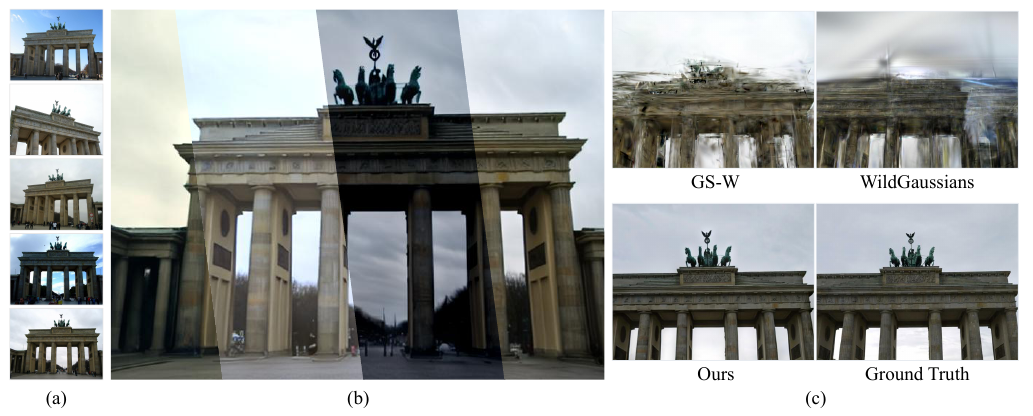
\includegraphics[width=0.72\textwidth]{figures/c_sgsw.png}
\caption{Trích từ SparseGS-W~\cite{sparsegsw}, Fig.~1: với 5 ảnh du lịch, GS-W và WildGaussians tạo artifact kéo dài.}
\end{figure}

\papersays
Tự nhận là ``first framework'' cho few-shot in-the-wild (§1). DUSt3R, Stable Diffusion 1.5 tinh chỉnh tăng cường ảnh góc nhìn mới, AdaIN theo ảnh tham chiếu. PSNR 19.01 so với 14.80 (GS-W) và 14.73 (WildGaussians) trên PhotoTourism 5 ảnh (Bảng~1).
\wesay
Tiên nghiệm nặng, không có mô-đun bù ngoại hình theo góc nhìn trong 3DGS, không đánh giá hình học.

\subsubsection{MS-GS~\cite{msgs}}
\info{Li và cộng sự (JHU, UCSD), NeurIPS 2025. Mip-NeRF 360, PhotoTourism (20 ảnh), tập drone 4 điều kiện thời tiết.}

\begin{figure}[H]
\centering
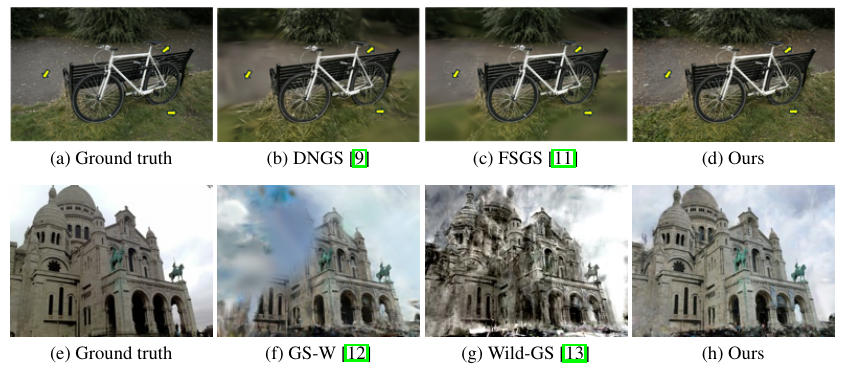
\includegraphics[width=0.72\textwidth]{figures/c_msgs.png}
\caption{Trích từ MS-GS~\cite{msgs}, Fig.~1: với ít ảnh và nhiều điều kiện ngoại hình, GS-W và Wild-GS có sai số lớn tại góc nhìn mới.}
\end{figure}

\papersays
Ít ảnh và nhiều điều kiện ngoại hình làm quá khớp nghiêm trọng hơn (§3.2); nhánh affine của WildGaussians hấp thụ sai số trắc quang (§4.4). Khởi tạo dày từ độ sâu theo vùng ngữ nghĩa và giám sát góc nhìn ảo; ablation: +0.80 dB và +0.58 dB (Bảng~1).
\wesay
Các nhận định định tính, không có chỉ số hình học, không tách biệt hai yếu tố.

\subsubsection{WildSplatter~\cite{wildsplatter}}
\info{Fujimura và cộng sự, arXiv 2604.21182. NeRF-OSR, 2--4 ảnh.}
\papersays
Feed-forward trên Depth Anything 3; hình học bất biến theo chiếu sáng, chỉ dự đoán màu theo embedding toàn cục.
\wesay
Không xét cơ chế hình thành floater trong tối ưu; chỉ dùng làm tham chiếu.

%=====================================================================
\section{Khoảng trống nghiên cứu và đóng góp dự kiến}
\label{sec:gap}

\begin{table}[H]
\centering\small
\caption{So sánh các nhóm công trình. ``Tách biệt hai yếu tố'': thí nghiệm có kiểm soát theo $N\times S$. Hàng cuối là mục tiêu, chưa phải kết quả.}
\label{tab:gap}
\begin{tabularx}{\textwidth}{@{}Y c c c c@{}}
\toprule
Công trình & Ít ảnh & Sai lệch trắc quang & Đánh giá hình học & Tách biệt hai yếu tố \\
\midrule
Nhóm A (8 công trình) & Có & Không & Không & Không \\
Nhóm B (trừ Appearance + Bilateral) & Không & Có & Không & Không \\
Appearance Codes + Bilateral Grids & Không & Có & Có (cần LiDAR) & Không \\
Gaussian-DK & Không (80--130 ảnh) & Có & Không & Không \\
SparseGS-W, MS-GS, WildSplatter & Có & Có & Không & Không \\
\midrule
\textbf{Đề xuất của nhóm} & \textbf{Có} & \textbf{Có (tổng hợp)} & \textbf{Có (GT của DTU)} & \textbf{Có} \\
\bottomrule
\end{tabularx}
\end{table}

\paragraph{Khoảng trống, theo thứ tự ưu tiên.}
\begin{description}[style=nextline]
  \item[G1 --- Thiếu đánh giá hình học (mạnh).] Gaussian-DK và các công trình nhóm C xử lý đồng thời sai lệch trắc quang và floater nhưng chỉ đánh giá bằng chỉ số ảnh; cơ chế floater bù trừ độ sáng được nêu dưới dạng giả định.
  \item[G2 --- Chưa tách biệt và định lượng tương tác (mạnh).] Chưa có thí nghiệm giai thừa $N\times S$; nhận định ``quá khớp nghiêm trọng hơn'' (MS-GS §3.2) chưa được định lượng.
  \item[G3 --- Quan hệ cải thiện trắc quang -- hình học (khá mạnh).] ICO-GS và MS-GS nêu khả năng ngoại hình bù trừ sai số hình học; chưa có đo lường đồng thời mức cải thiện trắc quang, mức cải thiện hình học và dung lượng mô-đun.
\end{description}
Giả thuyết về độ tin cậy của rendering disagreement dưới sai lệch trắc quang hệ thống (bản trước gọi là G4) được chuyển thành một thí nghiệm kiểm chứng cụ thể (E7) với CoR-GS.

\paragraph{Đóng góp dự kiến.}
\label{sec:contrib}
\begin{itemize}
  \item[\textbf{C1.}] \textbf{Benchmark hình học có kiểm soát:} giao thức trên DTU thay đổi độc lập $N$ và $S$, đánh giá trực tiếp bằng bề mặt tham chiếu (G1).
  \item[\textbf{C2.}] \textbf{Phân tích tương tác:} ước lượng tác động riêng và tương tác của $N$ và $S$ lên chỉ số floater (G2).
  \item[\textbf{C3.}] \textbf{Đánh đổi ngoại hình -- hình học:} với 1--2 mô-đun bù ngoại hình, đo đồng thời cải thiện trắc quang và cải thiện hình học (G3); kèm thí nghiệm E7 với CoR-GS. Kết quả E4 (bù affine theo ảnh, Mục~\ref{sec:factors}) cung cấp dữ liệu ban đầu cho C3.
\end{itemize}
Mô hình phân tích cho C2:
\begin{equation}
g(Y) = \beta_0+\beta_1N+\beta_2S+\beta_3\,N S+u_{\text{scan}}+\epsilon,
\end{equation}
trong đó $Y$ là chỉ số floater, $g$ là hàm logit (do $Y\in[0,1]$), $u_{\text{scan}}$ là hiệu ứng theo scan. Hệ số $\beta_3$ biểu thị tương tác. Do chỉ có ít scan, kết quả được báo cáo đồng thời theo từng scan, kèm phân tích hiệu theo cặp $\Delta_S(N)=Y(N,S)-Y(N,\text{none})$ cùng scan và seed.

%=====================================================================
\section{Giao thức đo và kết quả sơ bộ RQ1}
\label{sec:pilot}

\subsection{Giao thức}
\label{sec:protocol}
\begin{itemize}
  \item \textbf{Dữ liệu và chuẩn hoá.} DTU, ảnh 400$\times$300 (giảm 4 lần), mặt nạ vật thể. Cảnh được chuẩn hoá bằng ma trận \texttt{scale\_mat} của \texttt{cameras\_sphere.npz} (quy ước IDR/NeuS), đưa vật thể vào hình cầu bán kính xấp xỉ 1, áp dụng giống nhau cho mọi scan. Bề mặt tham chiếu là đám mây điểm STL chính thức của DTU, đã chuyển sang hệ toạ độ chuẩn hoá và lọc theo mặt nạ.
  \item \textbf{Chọn camera.} Tập huấn luyện được chọn bằng lấy mẫu điểm xa nhất (farthest-point sampling) tham lam trên tâm camera, xuất phát từ camera 0. Do tính tham lam, tập $N$ camera là tập con của tập $N'$ camera với $N<N'$ (tập lồng nhau). 16 góc nhìn kiểm định được chọn đều trong các camera còn lại.
  \item \textbf{Nhiễu trắc quang.} Chỉ áp dụng cho ảnh huấn luyện, trong mặt nạ vật thể:
  \begin{gather}
  I'_k = \operatorname{clip}(g_k\,\mathbf{w}_k \odot I_k)^{\gamma_k}, \\
  g_k = 2^{e_k},\ e_k\sim\mathcal{U}(-s,s);\quad
  \mathbf{w}_k = e^{\mathbf{u}_k},\ \mathbf{u}_k\sim\mathcal{U}(-b,b)^3;\quad
  \gamma_k = e^{v_k},\ v_k\sim\mathcal{U}(-\gamma,\gamma). \nonumber
  \end{gather}
  Mức none; mild $(s,b,\gamma)=(0.5,0.05,0.10)$; strong $(1.0,0.15,0.20)$. Tham số nhiễu xác định bởi seed nhiễu cố định.
  \item \textbf{Huấn luyện.} 7000 vòng lặp, mật độ hoá từ vòng 300 đến 3500, renderer PyTorch. \textbf{Khởi tạo: 10\,000 điểm ngẫu nhiên đều trong khối $[-1,1]^3$}, không dùng điểm SfM. \textbf{Màu RGB, SH bậc 0.} Gaussian có kích thước lớn hơn $0.1\times$ bán kính cảnh chỉ bị loại trong pha mật độ hoá (tới vòng 3500).
\end{itemize}

\subsection{Chỉ số}
Ký hiệu $d_i$ là khoảng cách từ tâm Gaussian $i$ tới điểm gần nhất của bề mặt tham chiếu (đơn vị chuẩn hoá; ngưỡng $\tau=0.1$ tương ứng khoảng 10\% bán kính hình cầu chuẩn hoá).
\begin{itemize}
  \item $\text{off}(\tau)=\frac{1}{N_G}\sum_i \mathbb{1}[d_i>\tau]$.
  \item \textbf{Chỉ số chính:}
  \begin{equation}
  W_{\text{float}}(\tau) = \frac{\sum_{k\in\mathcal{T}}\sum_{\mathbf{p}}\sum_{i:\,d_i>\tau} w_{ik}(\mathbf{p})}{\sum_{k\in\mathcal{T}}\sum_{\mathbf{p}}\sum_{i} w_{ik}(\mathbf{p})},
  \end{equation}
  với $\mathcal{T}$ là 16 góc nhìn kiểm định, tổng trên toàn bộ pixel; $w_{ik}(\mathbf{p})$ là trọng số trộn chính xác (renderer PyTorch, các đóng góp nhỏ hơn $1/255$ bị loại). Pixel không có Gaussian đóng góp (nền) không tham gia tổng.
  \item $\text{front}(\tau)$: trong số Gaussian có $d_i>\tau$, tỉ lệ có trung vị theo các góc nhìn huấn luyện của $z_{\text{Gauss}}-z_{\text{bề mặt}}$ nhỏ hơn $-0.03$ (nằm phía trước bề mặt).
  \item acc, comp: khoảng cách trung bình Gaussian $\to$ bề mặt và bề mặt $\to$ Gaussian, chỉ xét Gaussian có độ mờ $>0.05$.
  \item PSNR so với ảnh kiểm định gốc: \textbf{không dùng để kết luận} trong RQ1, do mô hình học từ ảnh đã biến đổi màu; đánh giá ngoại hình cần một giao thức trắc quang riêng.
\end{itemize}

\subsection{Giới hạn của chỉ số}
\label{sec:metric-limits}
\begin{itemize}
  \item Khoảng cách từ tâm là proxy: cần phân tích độ nhạy theo $\tau\in\{0.03, 0.05, 0.1, 0.15\}$. Script đo đã được mở rộng để xuất $\text{off}(\tau)$, $W_{\text{float}}(\tau)$, số lượng, tổng độ mờ và tổng đóng góp tuyệt đối của Gaussian vượt ngưỡng (không cần huấn luyện lại).
  \item Nếu tiến độ cho phép: tính khoảng cách cho các điểm lấy mẫu trong vùng hỗ trợ của Gaussian thay vì chỉ tâm.
\end{itemize}

\subsection{Kết quả sơ bộ}
\begin{figure}[H]
\centering
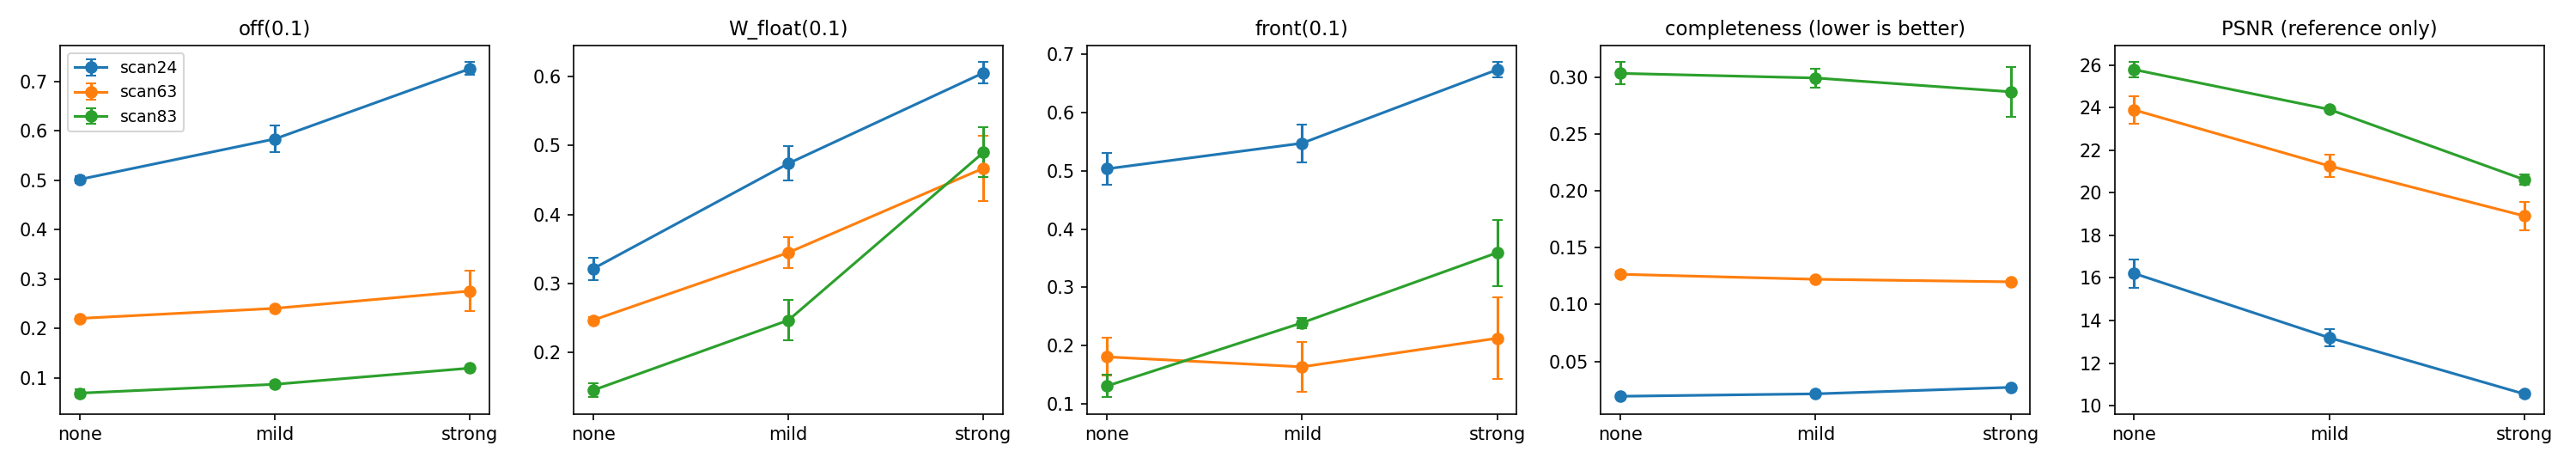
\includegraphics[width=\textwidth]{figures/dose_response.png}
\caption{Kết quả sơ bộ, $N=8$, đủ 27 lượt huấn luyện (3 scan $\times$ 3 mức $\times$ 3 seed). Từ trái sang phải: off(0.1), $W_{\text{float}}(0.1)$, front(0.1), completeness, PSNR. Điểm: trung bình theo seed; thanh sai số: độ lệch chuẩn mẫu.}
\end{figure}

\begin{table}[H]
\centering\small
\caption{Biến thiên so với mức none, so sánh theo cặp cùng scan và seed ($N=8$).}
\begin{tabular}{@{}lcccccc@{}}
\toprule
Mức & Số cặp & $\Delta W_{\text{float}}(0.1)$ & $\Delta\text{off}(0.1)$ & $\Delta$front(0.1) & $\Delta$acc & $\Delta$comp \\
\midrule
mild & 9 & $+0.117$ (9/9 tăng) & $+0.040$ (9/9) & $+0.045$ (7/9) & $+0.029$ (9/9) & $-0.002$ (5/9 tăng) \\
strong & 9 & $+0.283$ (9/9 tăng) & $+0.110$ (9/9) & $+0.144$ (8/9) & $+0.092$ (9/9) & $-0.005$ (3/9 tăng) \\
\bottomrule
\end{tabular}
\end{table}

\begin{table}[H]
\centering\small
\caption{$W_{\text{float}}(0.1)$ trung bình theo seed và tỉ số $W_{\text{float}}(0.1)/\text{off}(0.1)$ (mức đóng góp kết xuất tương đối của Gaussian vượt ngưỡng).}
\begin{tabular}{@{}lccc|ccc@{}}
\toprule
 & \multicolumn{3}{c|}{$W_{\text{float}}(0.1)$} & \multicolumn{3}{c}{$W_{\text{float}}/\text{off}$} \\
Scan & none & mild & strong & none & mild & strong \\
\midrule
scan24 & 0.321 & 0.474 & 0.606 & 0.64 & 0.81 & 0.83 \\
scan63 & 0.247 & 0.345 & 0.467 & 1.12 & 1.43 & 1.70 \\
scan83 & 0.145 & 0.247 & 0.490 & 2.11 & 2.82 & 4.08 \\
\bottomrule
\end{tabular}
\end{table}

\paragraph{Quan sát.}
\begin{itemize}
  \item $W_{\text{float}}(0.1)$ tăng đơn điệu theo $S$ trên cả ba scan và tăng ở toàn bộ 18 cặp so sánh (9/9 ở mỗi mức). off(0.03) cũng tăng đơn điệu (scan63: 0.45, 0.49, 0.56; scan83: 0.32, 0.34, 0.40), cho thấy xu hướng không phụ thuộc riêng vào ngưỡng 0.1. Kết quả \emph{phù hợp} với P1.
  \item Tỉ số $W_{\text{float}}/\text{off}$ tăng theo $S$ trên cả ba scan (scan83: 2.11 lên 4.08). Nghĩa là mức đóng góp kết xuất trung bình của mỗi Gaussian vượt ngưỡng tăng nhanh hơn số lượng của chúng: dưới sai lệch trắc quang, các Gaussian ngoài bề mặt không chỉ nhiều hơn mà còn xuất hiện rõ hơn trên ảnh. Quan sát này cho thấy chỉ đếm số lượng (off) đánh giá thấp mức độ floater.
  \item front(0.1) tăng ở 7/9 cặp (mild) và 8/9 cặp (strong); không đơn điệu ở scan63. P3 được ủng hộ một phần.
  \item Completeness hầu như không đổi trong khi accuracy suy giảm ở toàn bộ 18 cặp và số Gaussian tăng (trung bình $+3.1$ nghìn ở mild, $+12.4$ nghìn ở strong). Diễn giải ``mô hình bổ sung Gaussian ngoài bề mặt thay vì đánh mất bề mặt'' là hợp lý nhưng chưa đủ bằng chứng về cơ chế: số Gaussian tăng có thể một phần do mật độ hoá phản ứng với gradient lớn hơn~\cite{adgs}.
  \item Về thống kê: 18/18 cặp cùng chiều, nhưng các cặp không độc lập (cùng scan dùng chung cấu hình nhiễu; ba seed chỉ khác khởi tạo và tính ngẫu nhiên của huấn luyện). Không quy đổi thành giá trị $p$ cho tới khi có thêm scan và cấu hình nhiễu.
\end{itemize}

\subsection{Phân tích độ vững và cơ chế}
\label{sec:robust}
Các thí nghiệm trong mục này được thực hiện trên checkpoint hiện có (E0, E2b, E2c) hoặc với 18 lượt huấn luyện bổ sung (E6), $N=8$. Các thí nghiệm thay đổi biểu diễn màu, cấu trúc nhiễu và số góc nhìn (E5, E4, E1, E3) được trình bày ở Mục~\ref{sec:factors}.

\paragraph{E0 --- Độ nhạy theo ngưỡng.} $W_{\text{float}}(\tau)$ và off$(\tau)$ tăng đơn điệu none $<$ mild $<$ strong với cả bốn ngưỡng $\tau\in\{0.03, 0.05, 0.1, 0.15\}$ trên cả ba scan (24/24 so sánh). Ví dụ scan83: $W_{\text{float}}(0.03)$ từ 0.42 lên 0.70, $W_{\text{float}}(0.15)$ từ 0.08 lên 0.43. Kết luận P1 không phụ thuộc vào việc chọn $\tau=0.1$.

\paragraph{E0 --- Phân rã đóng góp ($\tau=0.1$).} Bảng~\ref{tab:decomp} so sánh mức strong với mức none.
\begin{table}[H]
\centering\small
\caption{Tỉ lệ strong/none (trung bình theo seed). ``Gần bề mặt'': Gaussian có $d\le 0.1$.}
\label{tab:decomp}
\begin{tabular}{@{}lccccc@{}}
\toprule
Scan & Số floater & Tổng độ mờ floater & Đóng góp floater & Đóng góp/floater & Đóng góp gần bề mặt \\
\midrule
scan24 & $\times 1.69$ & $\times 1.81$ & $\times 2.07$ & $\times 1.22$ & $\times 0.64$ \\
scan63 & $\times 1.71$ & $\times 1.42$ & $\times 2.22$ & $\times 1.29$ & $\times 0.82$ \\
scan83 & $\times 2.08$ & $\times 1.52$ & $\times 5.07$ & $\times 2.44$ & $\times 0.89$ \\
\bottomrule
\end{tabular}
\end{table}
Đóng góp của floater tăng nhanh hơn số lượng, trong khi đóng góp của các Gaussian gần bề mặt giảm: floater che bề mặt trên ảnh kiểm định chứ không chỉ cộng thêm vào. Chỉ đếm số lượng (off) đánh giá thấp mức độ floater; $W_{\text{float}}$ phản ánh đầy đủ hơn.

\paragraph{E2b --- Số góc nhìn quan sát mỗi floater.} Với mỗi Gaussian, $n_{\text{vis}}$ là số góc nhìn huấn luyện mà nó đóng góp trọng số trộn lớn hơn ngưỡng $\varepsilon$. Tỉ lệ mức tăng $W_{\text{float}}$ (none $\to$ strong) đến từ floater có $n_{\text{vis}}\le 2$:
\begin{table}[H]
\centering\small
\begin{tabular}{@{}lccc@{}}
\toprule
Scan & $\varepsilon=0.1$ & $\varepsilon=0.3$ & $\varepsilon=1.0$ \\
\midrule
scan24 & 0.91 & 0.91 & 0.95 \\
scan63 & 0.14 & 0.15 & 0.27 \\
scan83 & 0.01 & 0.02 & 0.04 \\
\bottomrule
\end{tabular}
\end{table}
Trên scan63 và scan83, mức tăng chủ yếu đến từ floater được \emph{nhiều} góc nhìn quan sát (scan83 mức strong: trung bình 4.1/8 góc nhìn với $\varepsilon=0.1$, nhiều hơn Gaussian bề mặt). Phát biểu ``floater chỉ nằm trong trường nhìn của một hoặc hai góc nhìn'' \textbf{không được ủng hộ} trên hai scan này. Khoảng cách trung bình (có trọng số) từ floater tới camera huấn luyện gần nhất chỉ giảm 4--8\%, do đó floater cũng không tập trung sát camera như mô tả của Gaussian-DK và VastGaussian. Kết quả này phù hợp với cơ chế (b) theo nghĩa thị sai: với SH bậc 0, Gaussian ngoài bề mặt quan sát được từ nhiều góc nhìn vẫn tạo ra sai khác phụ thuộc góc nhìn. scan24 cho kết quả ngược lại, phù hợp với nghi vấn về pipeline của scan này.

\paragraph{E2c --- Gaussian kích thước lớn.} Ở mức strong, khoảng 7 Gaussian mỗi mô hình có kích thước vượt ngưỡng cắt ($0.1\times$ bán kính cảnh), chiếm khoảng 34\% (scan63) và 23\% (scan83) mức tăng $W_{\text{float}}$. Các Gaussian này tồn tại được do không còn bước cắt kích thước sau vòng 3500. Kích thước trung vị và phân vị 99 của floater không đổi giữa các mức; phần còn lại của mức tăng đến từ floater kích thước bình thường với số lượng lớn hơn.

\paragraph{E6 --- Giữ cắt kích thước tới hết huấn luyện.} Huấn luyện lại scan63, scan83 (3 mức $\times$ 3 seed) với bước cắt Gaussian lớn được duy trì sau vòng 3500.
\begin{table}[H]
\centering\small
\caption{Mức tăng $\Delta W_{\text{float}}(0.1)$ so với none, có và không có cắt kích thước sau mật độ hoá.}
\begin{tabular}{@{}llccc@{}}
\toprule
Scan & Mức & Gốc & Có cắt kích thước & Tỉ lệ \\
\midrule
scan63 & mild & $+0.098$ & $+0.087$ (3/3 tăng) & 0.89 \\
scan63 & strong & $+0.220$ & $+0.187$ (3/3) & 0.85 \\
scan83 & mild & $+0.102$ & $+0.130$ (3/3) & 1.27 \\
scan83 & strong & $+0.345$ & $+0.353$ (3/3) & 1.02 \\
\bottomrule
\end{tabular}
\end{table}
Loại bỏ các Gaussian kích thước lớn chỉ làm mức tăng giảm 0--15\%, nhỏ hơn nhiều so với phần đóng góp 23--34\% của chúng trong cấu hình gốc. Vai trò của các Gaussian bị loại được thay thế bởi các Gaussian ngoài bề mặt khác. \textbf{P1 không phụ thuộc vào artifact này}. Quan sát cũng gợi ý rằng floater được hình thành do áp lực của phần dư trắc quang, không do một cơ chế huấn luyện cụ thể; đây là diễn giải, chưa được kiểm chứng trực tiếp.

\subsection{Biểu diễn màu, cấu trúc nhiễu và số góc nhìn}
\label{sec:factors}
Các thí nghiệm dưới đây sử dụng scan63 và scan83, 3 seed, cùng giao thức như Mục~\ref{sec:protocol}. Mức none của biến thể gốc (SH bậc 0, không bù ngoại hình) được dùng làm mốc khi biến thể không có mức none riêng (E1).

\paragraph{E5 --- SH bậc 3.} Thay màu RGB bằng hệ số SH bậc 3 (learning rate của các hệ số bậc $\ge 1$ bằng 1/20 learning rate màu, cộng trong miền logit).
\begin{table}[H]
\centering\small
\caption{$\Delta W_{\text{float}}(0.1)$ so với none của cùng biến thể.}
\begin{tabular}{@{}llcccc@{}}
\toprule
Scan & Mức & SH bậc 0 & SH bậc 3 & Tỉ lệ & $W_{\text{float}}$ strong: SH0 $\to$ SH3 \\
\midrule
scan63 & mild & $+0.098$ & $+0.093$ & 0.95 & \\
scan63 & strong & $+0.220$ & $+0.208$ & 0.95 & 0.467 $\to$ 0.438 \\
scan83 & mild & $+0.102$ & $+0.055$ & 0.54 & \\
scan83 & strong & $+0.345$ & $+0.235$ & 0.68 & 0.490 $\to$ 0.449 \\
\bottomrule
\end{tabular}
\end{table}
P1 vẫn đúng với SH bậc 3. Ở scan83, mức tăng nhỏ hơn chủ yếu do mức nền của SH bậc 3 cao hơn (0.214 so với 0.145), trong khi $W_{\text{float}}$ ở mức strong gần như không đổi. Với 15 hệ số bậc cao cho mỗi kênh, mô hình về nguyên tắc có thể khớp màu riêng cho 8 góc nhìn, nhưng vẫn hình thành Gaussian ngoài bề mặt. Giải thích ``floater xuất hiện vì không có kênh màu phụ thuộc hướng nhìn'' bị suy yếu; kết quả phù hợp hơn với giải thích rằng quá trình tối ưu và mật độ hoá ưu tiên giảm phần dư bằng hình học~\cite{adgs}. Diễn giải này phụ thuộc cấu hình: learning rate thấp có thể làm các hệ số SH học chậm hơn tốc độ mật độ hoá.

\paragraph{E4 --- Bù affine theo ảnh.} Mỗi ảnh huấn luyện có một ma trận $3\times3$ và vector độ lệch (12 tham số), khởi tạo bằng phép đồng nhất, áp lên ảnh kết xuất chỉ trong hàm mất mát; ảnh kiểm định được kết xuất không qua phép biến đổi này. Mô hình affine biểu diễn chính xác thành phần $g_k$ và $w_k$ của nhiễu, nhưng không biểu diễn được thành phần $\gamma_k$ (phi tuyến) và phép cắt.
\begin{table}[H]
\centering\small
\caption{$W_{\text{float}}(0.1)$ có và không có bù affine (SH bậc 0, $N=8$).}
\begin{tabular}{@{}llcccccc@{}}
\toprule
& & \multicolumn{2}{c}{$W_{\text{float}}$} & \multicolumn{2}{c}{$\Delta$ so với none} & \multicolumn{2}{c}{PSNR (dB)} \\
\cmidrule(lr){3-4}\cmidrule(lr){5-6}\cmidrule(lr){7-8}
Scan & Mức & Gốc & Affine & Gốc & Affine & Gốc & Affine \\
\midrule
scan63 & none & 0.247 & 0.242 & -- & -- & 23.89 & 24.24 \\
scan63 & mild & 0.345 & 0.318 & $+0.098$ & $+0.076$ & 21.26 & 22.30 \\
scan63 & strong & 0.467 & 0.405 & $+0.220$ & $+0.163$ & 18.91 & 20.05 \\
scan83 & none & 0.145 & 0.292 & -- & -- & 25.78 & 25.68 \\
scan83 & mild & 0.247 & 0.304 & $+0.102$ & $+0.012$ & 23.91 & 24.05 \\
scan83 & strong & 0.490 & 0.471 & $+0.345$ & $+0.179$ & 20.61 & 20.46 \\
\bottomrule
\end{tabular}
\end{table}
\begin{itemize}
  \item Bù affine \textbf{không} đưa $W_{\text{float}}$ về mức none. Ở mức strong, giá trị tuyệt đối chỉ giảm 13\% (scan63) và 4\% (scan83).
  \item Mức tăng $\Delta$ giảm 26--48\% ở mức strong. Tuy nhiên ở scan83, phần giảm này chủ yếu do mức nền tăng (0.145 $\to$ 0.292): khi dữ liệu không có nhiễu, mô-đun affine làm tăng floater. Kết quả này phù hợp với P4 (mô-đun ngoại hình có thể ảnh hưởng xấu tới hình học) nhưng cần thêm seed và scan để xác nhận.
  \item PSNR tăng khoảng 1 dB trên scan63, gần như không đổi trên scan83.
  \item Hai giải thích còn mở: (i) phần dư do $\gamma_k$ và phép cắt mà affine không biểu diễn được vẫn đủ gây floater; (ii) mô-đun affine và hình học được tối ưu đồng thời từ đầu, nên floater có thể hình thành trong giai đoạn mật độ hoá trước khi affine hội tụ. Hai giải thích này được tách bằng E4b (xem kế hoạch).
\end{itemize}
Lưu ý: mức none của scan83 dao động mạnh giữa các biến thể (0.145 với SH bậc 0, 0.214 với SH bậc 3, 0.292 với affine). Do đó các tỉ lệ $\Delta$ trên scan83 kém tin cậy hơn so sánh trực tiếp ở mức strong (0.45--0.49 ở cả ba biến thể).

\paragraph{E1 --- Nhiễu theo pixel không có hệ thống.} Giữ nguyên độ lớn sai lệch tại mỗi pixel như nhiễu ISP, nhưng đảo dấu ngẫu nhiên độc lập theo từng pixel: $I'=I+s\,(I^{\text{ISP}}-I)$, $s\in\{-1,+1\}$. Nhiễu có kỳ vọng bằng 0 và không còn thành phần nhất quán trong mỗi ảnh.
\begin{table}[H]
\centering\small
\caption{$\Delta W_{\text{float}}(0.1)$ so với none.}
\begin{tabular}{@{}llccc@{}}
\toprule
Scan & Mức & Nhiễu ISP & Nhiễu theo pixel & Tỉ lệ \\
\midrule
scan63 & mild & $+0.098$ & $+0.005$ & 0.05 \\
scan63 & strong & $+0.220$ & $+0.028$ & 0.13 \\
scan83 & mild & $+0.102$ & $-0.006$ & $-0.06$ \\
scan83 & strong & $+0.345$ & $-0.004$ & $-0.01$ \\
\bottomrule
\end{tabular}
\end{table}
Với cùng độ lớn sai lệch tại mỗi pixel, nhiễu không có hệ thống gần như không làm tăng floater. Yếu tố gây floater là \textbf{thành phần sai lệch nhất quán trong từng ảnh}, không phải độ lớn sai lệch theo điểm. Giới hạn: nhiễu theo pixel đồng thời loại bỏ tính nhất quán theo không gian và tính nhất quán trong ảnh; thí nghiệm này chưa tách được việc floater cần sai lệch \emph{khác nhau giữa các ảnh} hay chỉ cần sai lệch \emph{tần số thấp}. Đối chứng E1b (cùng một $\phi$ cho mọi ảnh) được đề xuất để tách hai trường hợp.

\paragraph{E3 --- Lưới $N\times S$.} $N\in\{4,6,8\}$, tập camera lồng nhau (FPS), 16 góc nhìn kiểm định cố định cho mọi $N$. Hình~\ref{fig:e3} trình bày kết quả.
\begin{figure}[H]
\centering
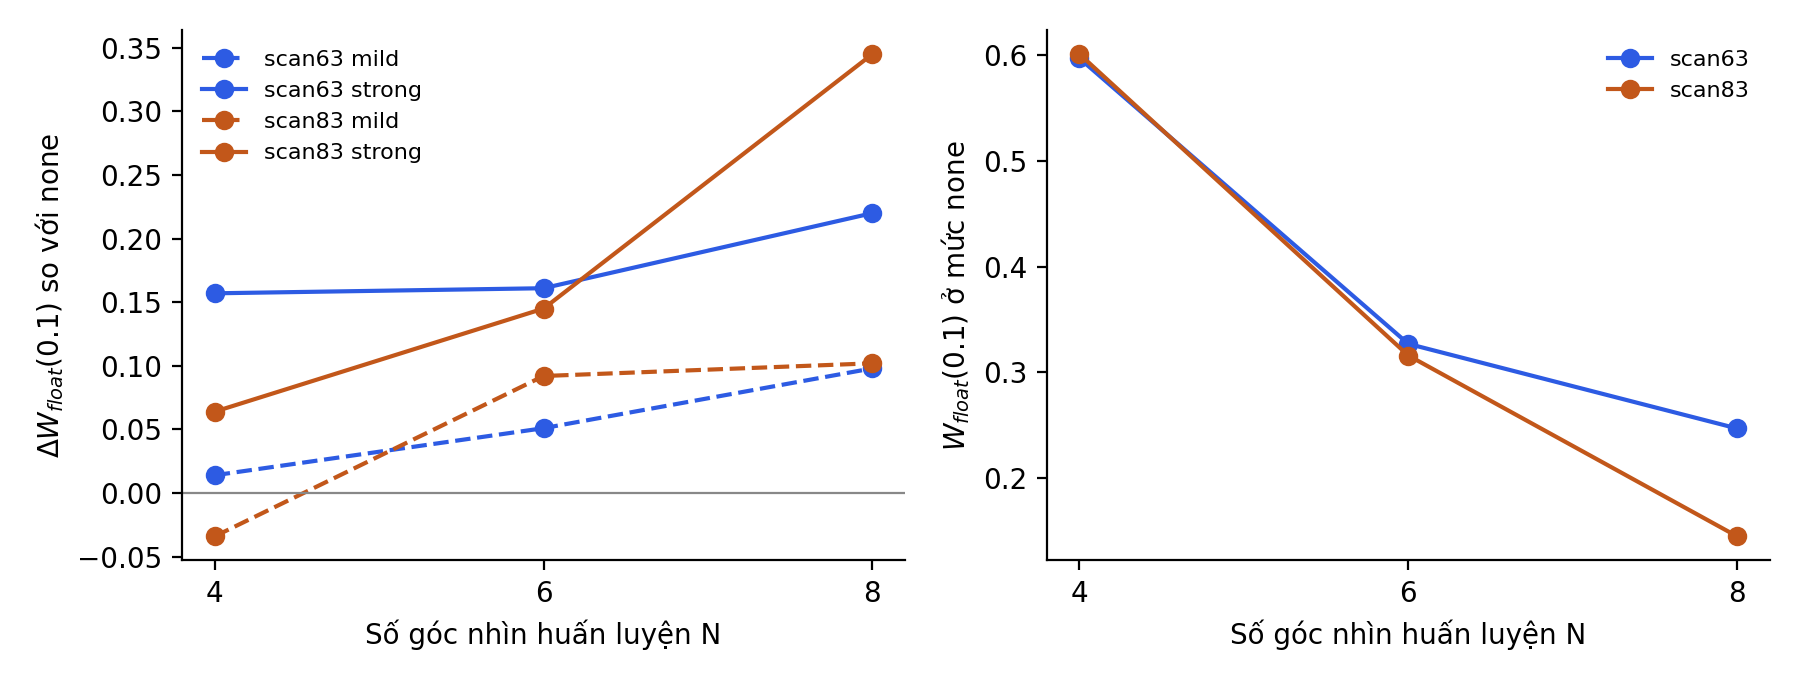
\includegraphics[width=0.95\textwidth]{figures/e3_interaction.png}
\caption{Trái: mức tăng $\Delta W_{\text{float}}(0.1)$ so với none theo $N$. Phải: $W_{\text{float}}(0.1)$ ở mức none. Trung bình 3 seed.}
\label{fig:e3}
\end{figure}
\begin{table}[H]
\centering\small
\caption{$\Delta W_{\text{float}}(0.1)$ so với none theo $N$.}
\begin{tabular}{@{}llccc@{}}
\toprule
Scan & Mức & $N=4$ & $N=6$ & $N=8$ \\
\midrule
scan63 & mild & $+0.014$ & $+0.051$ & $+0.098$ \\
scan63 & strong & $+0.157$ & $+0.161$ & $+0.220$ \\
scan83 & mild & $-0.034$ & $+0.092$ & $+0.102$ \\
scan83 & strong & $+0.064$ & $+0.145$ & $+0.345$ \\
\midrule
\multicolumn{2}{@{}l}{$W_{\text{float}}$ none (scan63 / scan83)} & 0.60 / 0.60 & 0.33 / 0.32 & 0.25 / 0.15 \\
\bottomrule
\end{tabular}
\end{table}
Hồi quy logit với hiệu ứng cố định theo scan ($S=0;\ 0.5;\ 1$): $\hat\beta_N=-0.449\pm0.039$, $\hat\beta_S=-0.46\pm0.38$, $\hat\beta_{NS}=+0.216\pm0.061$. Tác động của $S$ trên thang logit tại $N=4, 6, 8$ lần lượt là 0.40, 0.83, 1.27.
\begin{itemize}
  \item Giảm $N$ làm tăng floater mạnh (mức none từ khoảng 0.15--0.25 lên 0.60), phù hợp với các công trình nhóm A.
  \item \textbf{P2 không được ủng hộ}: trong khoảng $N=4$--8, tác động của sai lệch trắc quang \emph{tăng} theo $N$, ngược với dự đoán. Xu hướng xuất hiện ở cả hai scan và cả hai mức, và vẫn còn trên thang logit (thang đã hiệu chỉnh một phần hiệu ứng trần).
  \item Diễn giải đề xuất (chưa kiểm chứng): sai lệch trắc quang gây floater thông qua \emph{xung đột} giữa các góc nhìn cùng quan sát một vùng bề mặt. Khi $N$ nhỏ, vùng chồng lấn ít, phần dư của từng ảnh có thể được khớp trên bề mặt mà không xung đột, và floater chủ yếu do thiếu ràng buộc hình học. Khi $N$ tăng, hình học được ràng buộc chặt hơn và sai lệch trắc quang trở thành nguồn xung đột chính. Diễn giải này phù hợp với E2b (floater được trung bình khoảng 4/8 góc nhìn quan sát).
  \item Giới hạn: ở $N=4$, PSNR chỉ 11.8--16.3 dB và $W_{\text{float}}\approx0.6$ ngay ở mức none, nên đây là chế độ tái tạo suy biến; độ lệch chuẩn của hồi quy chưa tính tương quan giữa các lượt cùng seed; chỉ có hai scan; khoảng $N$ hẹp. Cần mở rộng tới $N\in\{12, 16\}$ để biết tác động của $S$ tiếp tục tăng hay đạt cực đại.
\end{itemize}

\paragraph{Kiểm tra scan24.} 98\% điểm tham chiếu nằm trong mặt nạ và mặt nạ được bề mặt tham chiếu phủ 89\%; không phát hiện lỗi pipeline. Khác biệt đến từ hình học camera: khoảng cách camera tới tâm là 2.89 (khoảng 5.0 ở hai scan còn lại), vật thể chiếm 62\% ảnh, và khối khởi tạo ngẫu nhiên $[-1,1]^3$ nằm một phần giữa vật thể và camera; 44\% floater có bán kính $r>1.2$. scan24 được báo cáo riêng và chỉ so sánh lại sau khi có điều kiện khởi tạo bằng điểm SfM.

\paragraph{Bề mặt tham chiếu chứa điểm ngoài mặt nạ.} Bề mặt tham chiếu được lọc với điều kiện ``nằm trong mặt nạ ở ít nhất 1 góc nhìn''. Tỉ lệ điểm tham chiếu nằm trong mặt nạ chỉ là 0.83 (scan63) và 0.62 (scan83). Hệ quả: completeness bị đánh giá cao, và Gaussian nằm gần các điểm tham chiếu ngoài vật thể bị tính là ``gần bề mặt'', dẫn tới đánh giá thấp $W_{\text{float}}$. Do các so sánh đều theo cặp, chiều của $\Delta$ khó thay đổi, nhưng độ lớn có thể thay đổi. Đề xuất lọc lại với điều kiện nằm trong mặt nạ ở ít nhất 80\% số góc nhìn quan sát được và tính lại E0 trên checkpoint hiện có.

\subsection{Tổng hợp trạng thái giả thuyết}
\begin{table}[H]
\centering\small
\caption{Trạng thái các giả thuyết sau E0--E6.}
\begin{tabularx}{\textwidth}{@{}p{4.2cm} Y p{3.2cm}@{}}
\toprule
Giả thuyết & Kết quả & Trạng thái \\
\midrule
P1 & Tăng ở 18/18 cặp; vững theo $\tau$, $\varepsilon$, khi loại Gaussian lớn, với SH bậc 3 và khi có bù affine & Được ủng hộ \\
P2 & Tác động của $S$ tăng theo $N$ trong khoảng 4--8 ($\hat\beta_{NS}>0$) & Không được ủng hộ \\
P3 & front(0.1) tăng ở 15/18 cặp; khoảng cách tới camera giảm ít & Ủng hộ một phần \\
P4 & Affine tăng PSNR ở scan63, giảm floater ít, tăng mức nền ở scan83 & Có dấu hiệu, cần thêm dữ liệu \\
(b), dạng ``chỉ 1--2 góc nhìn'' & Mức tăng đến từ floater được nhiều góc nhìn quan sát & Không được ủng hộ \\
Thiếu kênh màu phụ thuộc hướng nhìn & SH bậc 3 giữ 54--95\% mức tăng & Bị suy yếu \\
Thành phần nhất quán trong ảnh gây floater & Nhiễu theo pixel cùng độ lớn: mức tăng $\approx 0$ & Được ủng hộ (chưa có E1b) \\
Bù ngoại hình toàn cục loại bỏ floater & Affine giảm $W_{\text{float}}$ ở mức strong 4--13\% & Không được ủng hộ \\
\bottomrule
\end{tabularx}
\end{table}

\paragraph{Các yếu tố gây nhiễu đã nhận diện.}
\begin{enumerate}
  \item \textbf{Khởi tạo ngẫu nhiên} trong $[-1,1]^3$: một phần floater ở mức none xuất phát từ khởi tạo, đặc biệt ở scan24. So sánh theo cặp loại trừ ảnh hưởng này khỏi $\Delta$, nhưng giá trị tuyệt đối và tương tác với $N$ có thể bị ảnh hưởng. Đề xuất bổ sung khởi tạo bằng điểm SfM.
  \item \textbf{Bề mặt tham chiếu} chứa điểm ngoài mặt nạ (62--83\% điểm trong mặt nạ).
  \item \textbf{Dao động mức nền} ở scan83 (0.145--0.292 giữa các biến thể); chỉ có 3 seed.
  \item \textbf{Một cấu hình nhiễu} (seed 0): phân bố tham số nhiễu giữa các góc nhìn chưa thay đổi.
  \item \textbf{Hai scan} cho E1--E5; khoảng $N$ hẹp; $N=4$ là chế độ suy biến.
\end{enumerate}

\paragraph{Kế hoạch tiếp theo.}
\begin{enumerate}
  \item Lọc lại bề mặt tham chiếu và tính lại E0 trên checkpoint hiện có (không huấn luyện lại).
  \item E1b: cùng một $\phi$ cho mọi ảnh huấn luyện (12 lượt). Nếu floater không tăng, yếu tố gây floater là sai lệch \emph{khác nhau giữa các ảnh}.
  \item E4b: nhiễu chỉ gồm $g_k, w_k$ ($\gamma=0$) kèm bù affine, và bù affine được khởi động trước giai đoạn mật độ hoá; tách hai giải thích (i) và (ii) của E4.
  \item E3b: $N\in\{12, 16\}$ để xác định dạng tương tác.
  \item Khởi tạo bằng điểm SfM cho một tập con cấu hình.
  \item Khảo sát dataset có chiếu sáng vật lý (tiêu chí tại \texttt{docs/tasks/dataset\_survey\_criteria.md}).
\end{enumerate}

%=====================================================================
\begin{thebibliography}{99}\small
\bibitem{nerfw} R.~Martin-Brualla et al. NeRF in the Wild: Neural Radiance Fields for Unconstrained Photo Collections. CVPR 2021. arXiv:2008.02268.
\bibitem{fnm} J.~Philip, V.~Deschaintre. Floaters No More: Radiance Field Gradient Scaling for Improved Near-Camera Training. 2023. arXiv:2305.02756.
\bibitem{sparsegs} H.~Xiong et al. SparseGS: Sparse View Synthesis using 3D Gaussian Splatting. arXiv:2312.00206.
\bibitem{fsgs} Z.~Zhu, Z.~Fan, Y.~Jiang, Z.~Wang. FSGS: Real-Time Few-shot View Synthesis using Gaussian Splatting. ECCV 2024. arXiv:2312.00451.
\bibitem{dngaussian} J.~Li et al. DNGaussian: Optimizing Sparse-View 3D Gaussian Radiance Fields with Global-Local Depth Normalization. CVPR 2024. arXiv:2403.06912.
\bibitem{corgs} J.~Zhang et al. CoR-GS: Sparse-View 3D Gaussian Splatting via Co-Regularization. ECCV 2024. arXiv:2405.12110.
\bibitem{adgs} G.~Patle, N.~Girgaonkar, N.~Somraj, R.~Soundararajan. AD-GS: Alternating Densification for Sparse-Input 3D Gaussian Splatting. ACM TOG (SIGGRAPH Asia) 2025. doi:10.1145/3757377.3763993. arXiv:2509.11003.
\bibitem{icogs} K.~Xiong et al. Intrinsic Geometry-Appearance Consistency Optimization for Sparse-View Gaussian Splatting. CVPR 2026. arXiv:2603.02893.
\bibitem{herogs} J.~Li et al. HeroGS: Hierarchical Guidance for Robust 3D Gaussian Splatting under Sparse Views. arXiv:2603.01099, 2026.
\bibitem{vastgaussian} J.~Lin et al. VastGaussian: Vast 3D Gaussians for Large Scene Reconstruction. CVPR 2024. arXiv:2402.17427.
\bibitem{bilarf} Y.~Wang, C.~Wang, B.~Gong, T.~Xue. Bilateral Guided Radiance Field Processing. ACM TOG (SIGGRAPH) 2024. arXiv:2406.00448.
\bibitem{wildgaussians} J.~Kulhanek et al. WildGaussians: 3D Gaussian Splatting in the Wild. NeurIPS 2024. arXiv:2407.08447.
\bibitem{unifying} N.~Wang et al. Unifying Appearance Codes and Bilateral Grids for Driving Scene Gaussian Splatting. arXiv:2506.05280.
\bibitem{luminancegs} Z.~Cui, X.~Chu, T.~Harada. Luminance-GS: Adapting 3D Gaussian Splatting to Challenging Lighting Conditions with View-Adaptive Curve Adjustment. CVPR 2025.
\bibitem{gaussiandk} S.~Ye, Z.-H.~Dong, Y.~Hu, Y.-H.~Wen, Y.-J.~Liu. Gaussian in the Dark: Real-Time View Synthesis From Inconsistent Dark Images Using Gaussian Splatting. Computer Graphics Forum 43(7), Pacific Graphics 2024. doi:10.1111/cgf.15213. arXiv:2408.09130.
\bibitem{sparsegsw} Y.~Li et al. SparseGS-W: Sparse-View 3D Gaussian Splatting in the Wild with Generative Priors. arXiv:2503.19452, 2025.
\bibitem{msgs} D.~Li et al. MS-GS: Multi-Appearance Sparse-View 3D Gaussian Splatting in the Wild. NeurIPS 2025.
\bibitem{wildsplatter} Y.~Fujimura et al. WildSplatter: Feed-forward 3D Gaussian Splatting with Appearance Control from Unconstrained Images. arXiv:2604.21182, 2026.
\end{thebibliography}

\end{document}
